\setRL
%\pagenumbering{arabic} 


\section{\label{sec:cellmembrane}
غشای سلولی
}
غشاها ساختارهای زیستی هستند که در سامانه‌هایِ مختلفِ زیستیِ سلول‌هایِ هسته‌دار و بی هسته  نقش دارند. غشا در واقع دیوار یا مانعی‌است که مرز داخل و خارج سلول را مشخص می‌کند. همچنین در سلول‌های هسته‌دار، غشای هسته اورگان‌های خیلی مهم سلول را در خود جا می‌دهد. به عنوان مرز سلول با دینای خارج، غشا نقش مهمی در مدیریتِ نقل و انتقال مواد بین سلول و محیط پرامون دارد. درون غشا پروتئین‌ها، لیگاند‌ها
\LTRfootnote{ligand} 
،
و ملکول‌های درشت خیلی زیادی وجود دارد که در طیف‌ گسترده‌ای از فرآیندها از سیگنال‌دادن تا تقسیم سلولی نقش دارند.
\begin{figure}[h]
\begin{center}
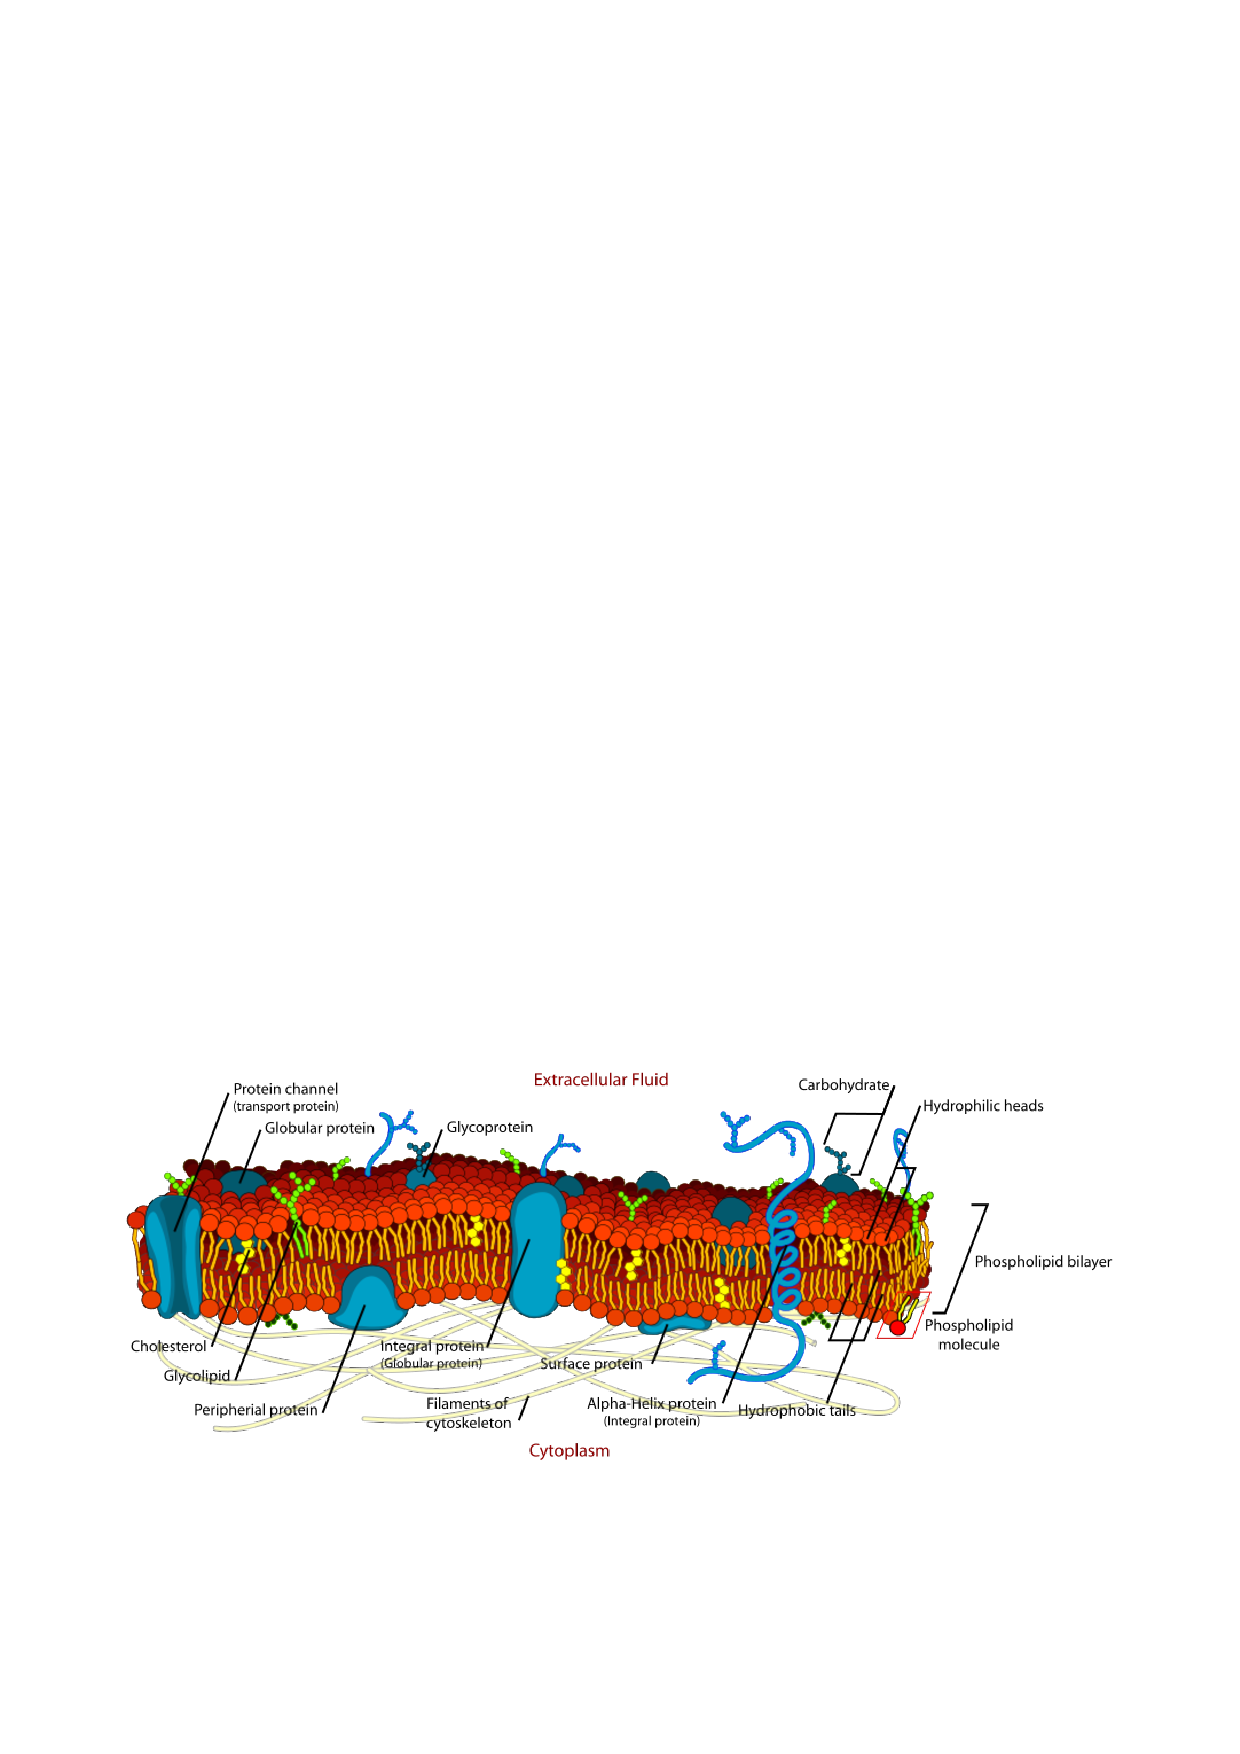
\includegraphics[width=4in]{\MemBio /Pics/Cell_membrane_detailed_diagram}
\caption{
شکل از سایت ویکیپیدیا گرفته شده است
\cite{wikiCellMembrane}
. این یک نقاشی از غشا بر اساس مدل غشای مایع موزایکی است. بیشتر غشا از ملکول‌های چربی تشکیل شده ولی پروتئین‌های خیلی زیادی نیز در غشا قرار دارد.  غشا از طریق این پروتئین‌ها به اسکلت سلولی و اجزای دیگر متصل است. دایره‌های قرمز سر آب دوست و رشته‌های زرد دم‌های آب گریز لیپید‌ها را نشان می‌دهد.
}
\label{fig:fluidmembranemodel}
\end{center}
\end{figure}

حاصل زحمات افراد در قرن ۱۹ و ۲۰ میلادی در راستای پی بردن به ساز و کار واحد‌های سازنده‌ی موجودات زنده، تصویری با جزئیات زیاد از سلول‌های زنده است. در سال ۱۹۸۵ ارنست اُورتن 
\LTRfootnote{Ernest Overton}  
سلول‌های گیاهی را در محلول‌های مختلف (قند،‌ الکل، اتر، فنول، و استن
\LTRfootnote{sugar, alcohols, ether, phenol, and acetone}
) قرار داد. مشاهدات وی نشان داد که (تحت اختلاف فشار اسمزی یکسان) محلول‌هایی مانند قند که در آب به راحتی حل می‌شوند نمی‌توانند وارد سلول شوند در صورتی که محلول‌های دیگری که حل شونده‌ی خوبی در آب نیستند، می‌توانند وارد سلول شوند. او نتیجه گرفت که جنس مرز سلول با سیتوپلاسم درون آن متفاوت است و به احتمال زیاد از ملکول‌های چربی گون تشکیل شده است
\cite{overton1985}
. در سال ۱۹۳۲ (حدود صد سال پیش) کِنِت کول
 \LTRfootnote{Kenneth Cole}
 تخم جوجه‌تیغی دریایی
 \LTRfootnote{sea urchin (arbacia) egg} 
را بر سطحی قرار داد و  با کمک یک فیبرِ از جنس طلا به تخم  فشار وارد کرد. با اندازه‌گیری  کشش سطحی و مقایسه‌ی آن با حد تحمل فشار تخم، استدلال کرد که لایه‌ی نازکی که در اطراف سلول وجود دارد تنها از ملکول‌های چربی درست نشده است
 \cite{Cole1932}
. در دهه‌ی ۱۹۵۰ با فرا رسیدن تکنولوژی میکروسکوپ الکترونی، اولین تصاویر از غشای سلول رونمایی شد و با استفاده از روش‌های رنگ آمیزی، وجود لیپید‌ها
\LTRfootnote{lipid}
 در غشا تایید و ضخامت غشای سلولی بین ۵ تا ۱۰ نانومتر اندازه‌گیری شد
\cite{ROBERTSON1959aa}
.


افراد زیادی در تکمیل تصویری که از غشای سلول هست نقش داشتند، ولی تصویر مدرنی که امروز از غشاهای سلول‌ها داریم، بیشتر بر پایه‌ی مدل غشای مایع موزایکی‌
\LTRfootnote{the mosaic fluid model of membranes}
 است که در سال ۱۹۷۲ توسط سینگر
 \LTRfootnote{Singer}
  و نیکلسون
  \LTRfootnote{Nicholson}
 ارائه شد
\cite{Singer1972}
(شکل 
\ref{fig:fluidmembranemodel}
). بنا بر این مدل، غشا را می‌توان یک مایع دو بعدی فرض کرد که در آن چربی‌ها و پروتئین‌ها می‌توانند کم و بیش آزادانه حرکت کنند. در نتیجه هیچ نظم بلند بردی در غشا دیده نمی‌شود. با وجود اینکه غشای چربی به طور خود سامانده تشکیل می‌شود ولی علاوه بر ملکول‌های چربی پروتئین‌های زیادی نیز به غشا ساختار می‌بخشد
\cite{wikiCellMembrane}
. غشا از طریق این پروتئین‌ها به اجزای پیچیده‌تر داخل سلول (مانند اسکلت سلولی) متصل است. خاصیت تراوایی فوسفولیپید دو لایه و کانال‌های پروتئینی درون غشا، ارتباط سلول با محیط اطراف را کنترل و مدیریت می‌کند. 







 
% \begin{figure}[h]
%\begin{center}
%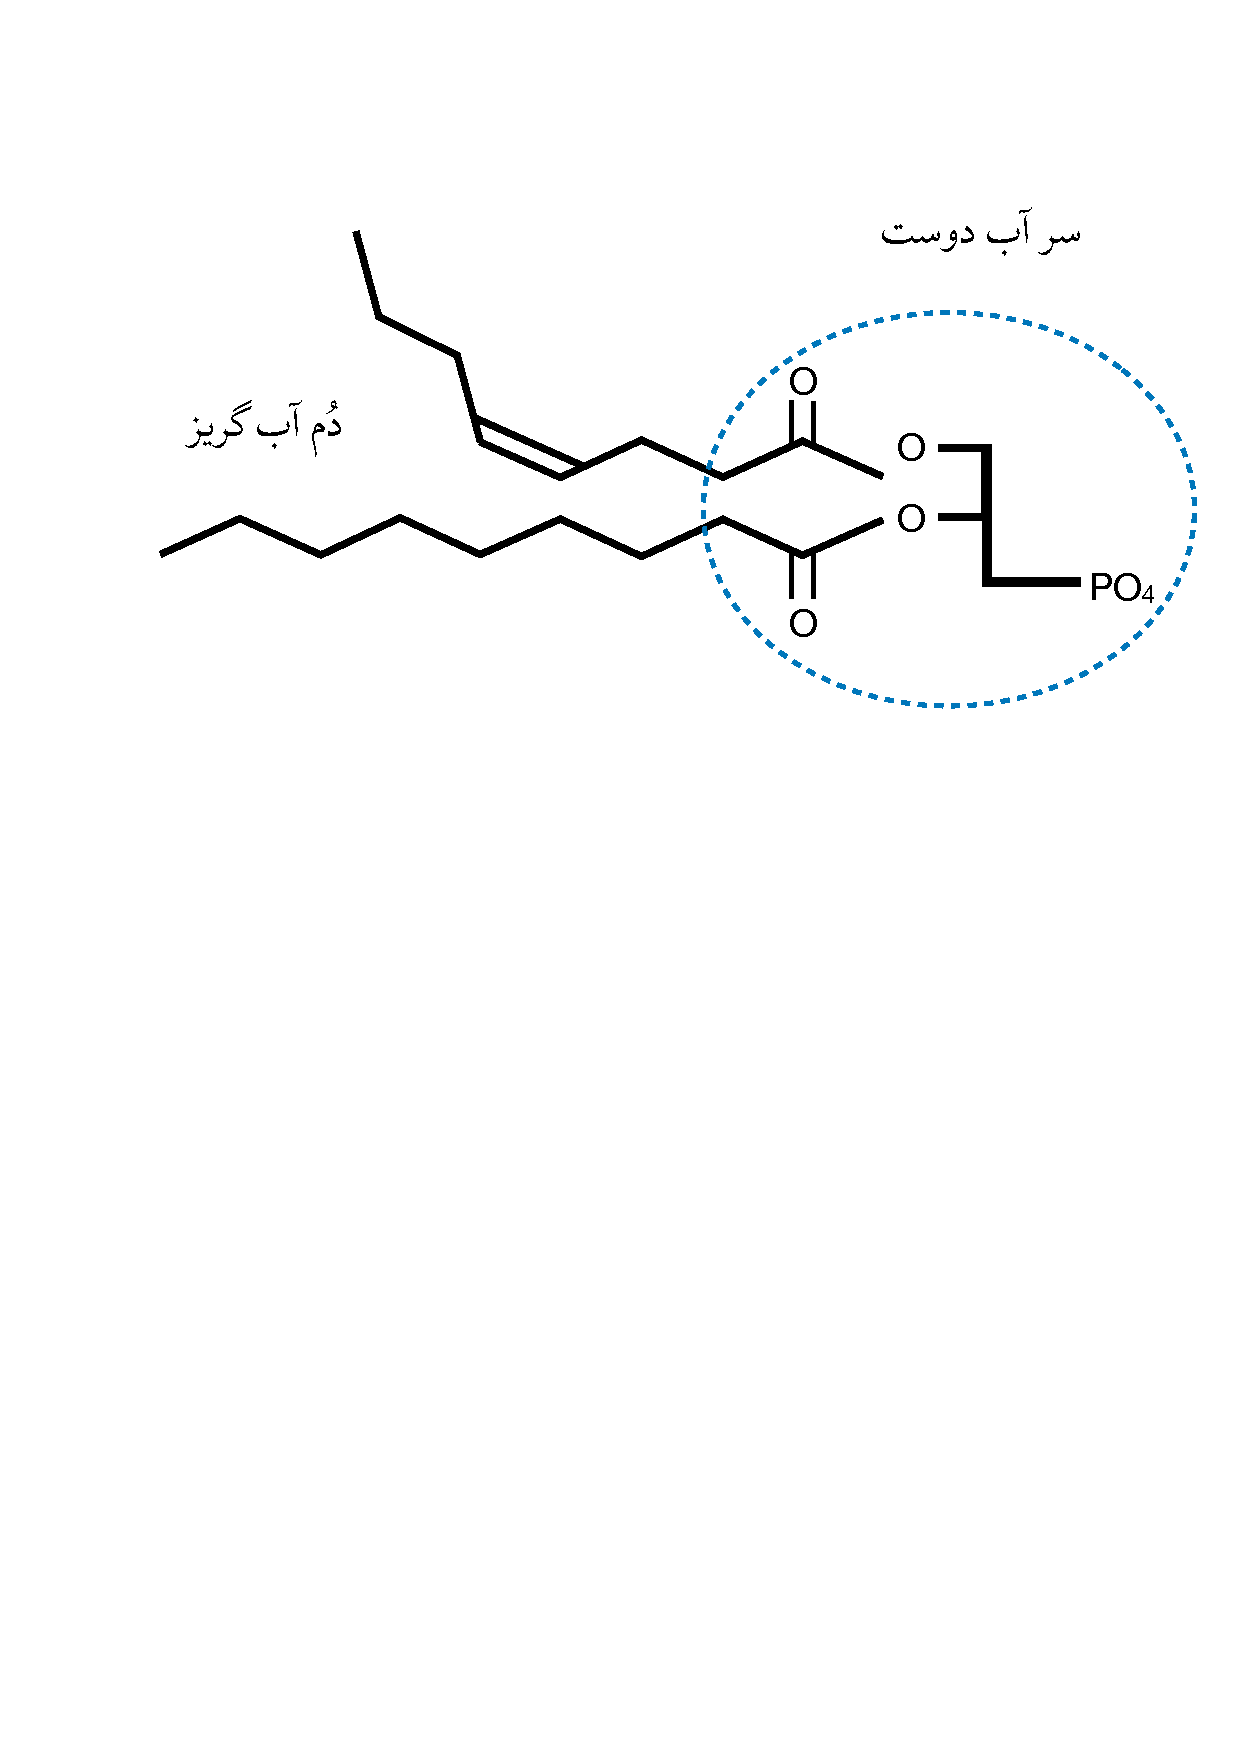
\includegraphics[width=4in]{\MemBio /Pics/Phospholipid}
%\caption{
%ساختار شیمیایی یک ملکول فوسفولیپید. سر آب دوست (دایره‌ی آبی) و  انتهای آبگریز مشخص شده است.
%}
%\label{fig:phospholipid}
%\end{center}
%\end{figure}
 
 
ملکول‌های لیپید یا چربی یکی از ۴ عناصری است که در کنار آمینو اسید‌ها، نوکلئیک اسید‌ها، و ملکول‌های قندی ساختار موجودات زنده را تشکیل می‌دهد
\cite{Membraneasamatteroffat}
.  بیش از هزار نوع ملکول چربی در گونه‌های زیستی وجود دارد ولی ساختار کلی آنها بسیار مشابه است. در سلول‌ پستانداران بیشتر فسفولیپید و گلیسرول یافت می‌شود. ملکول‌ فوسفولیپید از یک سر آب دوست
\LTRfootnote{hydrophilic}  
 و یک دُم آب گریز
 \LTRfootnote{hydrophobic}  
 ساخته شده‌است (شکل
\ref{fig:bilayer}
). فرق بین ملکول‌های لیپید مختلف در ساختار شیمایی سر آب دوست و دُم آب‌ گریز آنهاست. این ملکول‌ها در محلول‌های آبی
\textbf{بدون ایجاد پیوندها شیمیایی}
، به طور خود سامانده
  \LTRfootnote{self-assembly}  
 سطوح بزرگ دولایه تشکیل می‌دهند.  دُم‌های  آبگریز در مرکز لایه (به دور از آب) و سر آب دوست به سمت محلول جهت‌گیری می‌کند (شکل
\ref{fig:bilayer}
 ).
\begin{figure}[h]
\begin{center}
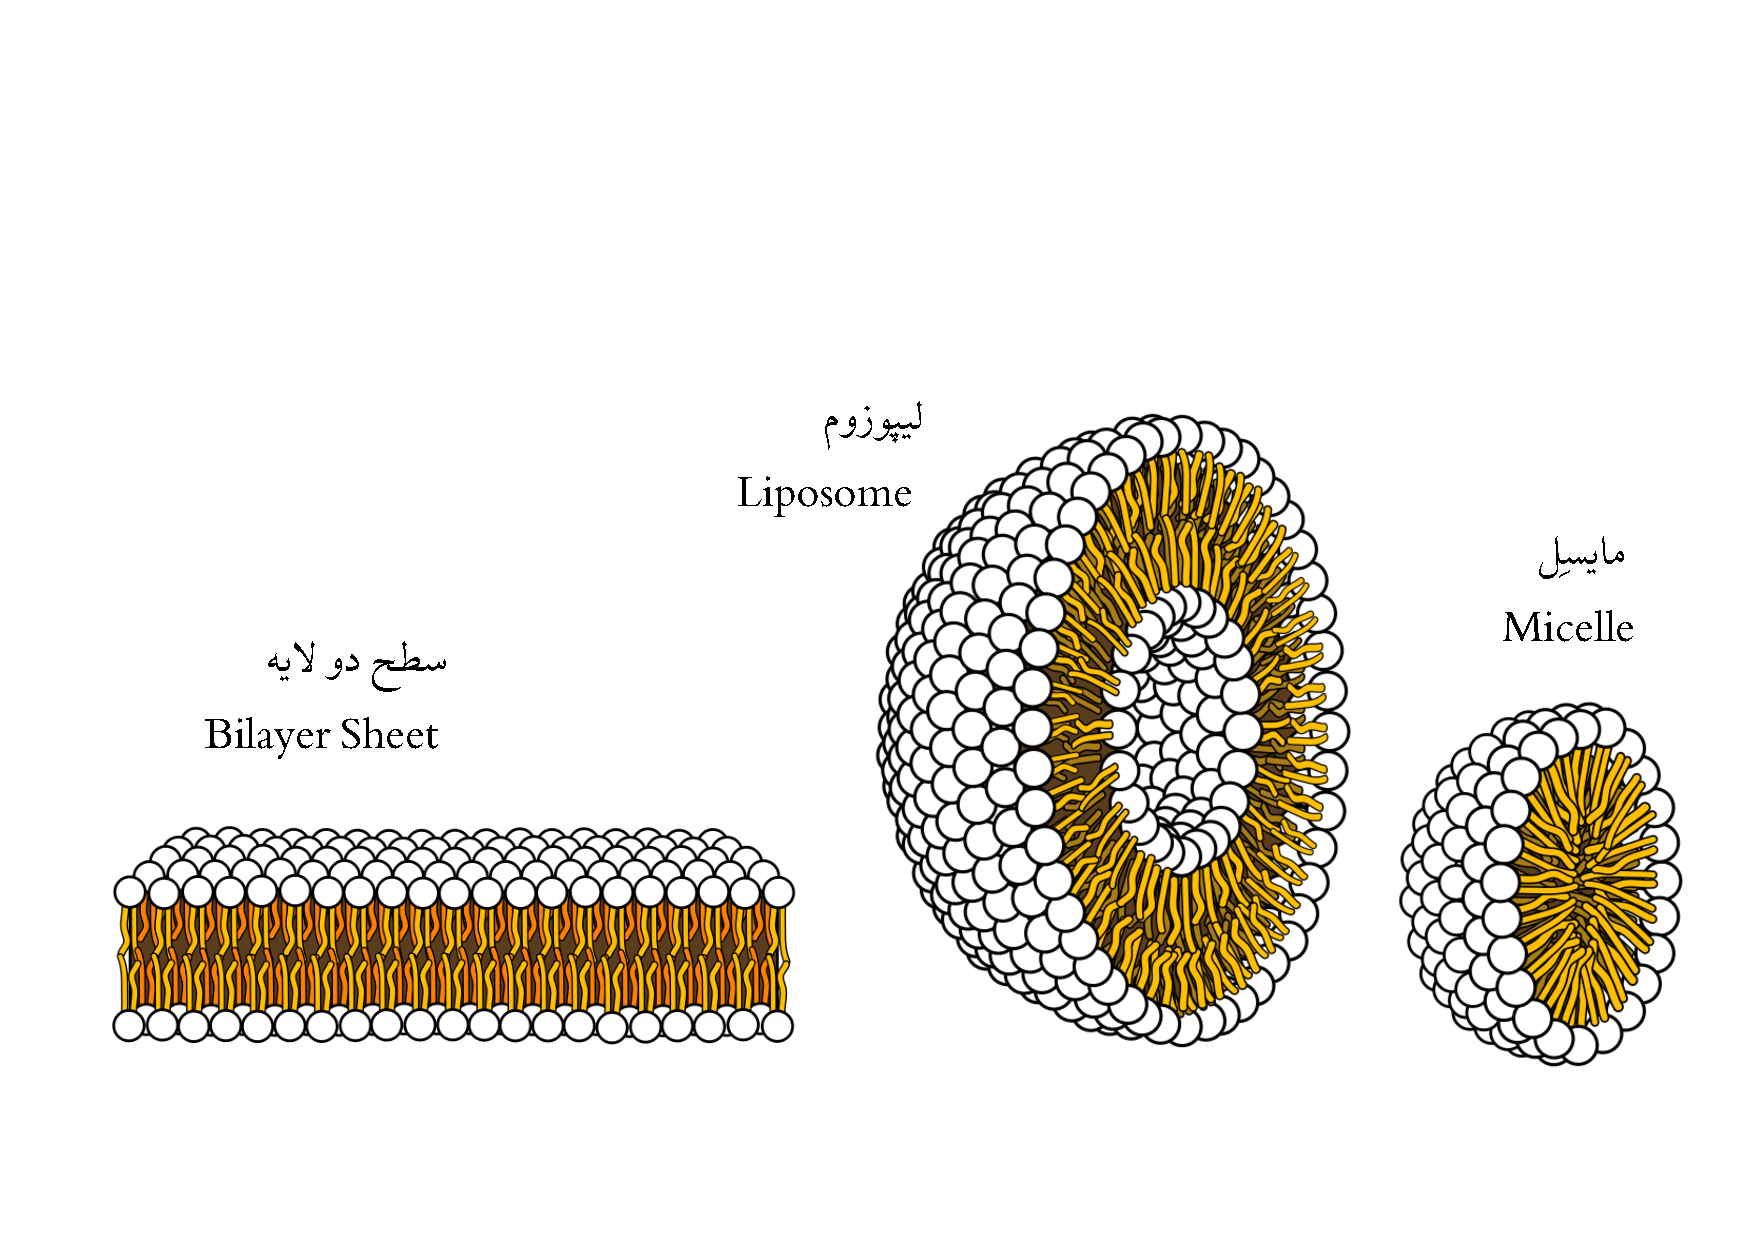
\includegraphics[width=4in]{\MemBio /Pics/Bilayer}
\caption{
الف) ساختار شیمیایی یک ملکول فوسفولیپید. سر آب دوست (دایره‌ی آبی) و  انتهای آبگریز مشخص شده است. ب) ساختار‌های معمول ملکول‌های چربی در آب. به ترتیب از چپ به راست، ساختار سطوح بزرگ دو لایه، کره‌های دو لایه (لیپوزوم)، و کره‌های کوچک تک لایه، مایسِل.
}
\label{fig:bilayer}
\end{center}
\end{figure}

\begin{figure}[h]
\begin{center}
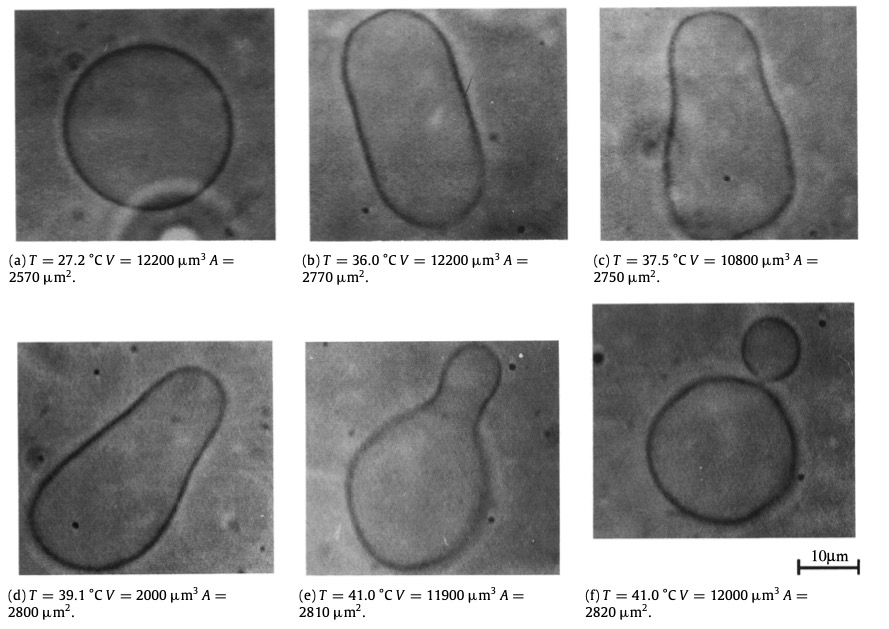
\includegraphics[width=4in]{\MemBio /Pics/GUVTempChange}
\caption{
تغییر ساختار یک غشای غول ‌آسا به علت تغییر دما از ۲۷/۲ تا ۴۱ درجه‌ی سانتیگراد. در دمای ۳۶ درجه حالت بیضی شکل، بالاتر از دمای ۳۶ شکل گلابی، و با ماندن در دمای ۴۱ درجه یک حباب بر روی آن جدا شده.
}
\label{fig:GUVTempChange}
\end{center}
\end{figure}
در نتیجه‌ی توسعه‌ی تحقیقات ما می‌دانیم غشا‌های زیستی بیشتر ساختار موزائیکی دارند تا مایع. یعنی در سلول‌های مختلف غشا خیلی همگن نیست و در یک سلول قسمت‌هایی از غشا ممکن است  ترکیب پروتئینی متفاوتی از بخش‌های دیگر همان سلول داشته باشد. همچنین ضخامت برخی از بخش‌های غشا ممکن است از چند ۱۰ نانومتر تا ۱۰۰ نانومتر تغییر کند
\cite{Engelman:2005aa}
. سلول‌هایی هم می‌توان یافت که درصد پروتئین و کربوهیدارت در ساختار غشای آن به ترتیب بین ۱۸ تا ۷۵ درصد و  ۳ تا ۱۰ درصد باشد
\cite{MembraneProteins1972}
. محققان با مطالعه‌ی غشا‌های غول‌آسا
\LTRfootnote{Giant Unilamellar vesicle}  
 یا 
 GUV اطلاعات  زیادی راجع به ساماندهی غشاهای چربی جمع‌آوری کرده‌اند. این غشا‌ها را معمولا می‌توان با  مخلوط کردن 
\LTRfootnote{mixing}  
 غشا‌ و ترکیب‌های چربی در آزمایشگاه ساخت
 \cite{GUVmaking2009}
و اندازه‌ی آن  از چند میلی‌متر تا چند میکرون  است. 
GUV نسبت به تغییرات ترمودینامیکی محیط واکنش‌های بسیار جالبی نشان می‌دهد. برای مثال شکل
\ref{fig:GUVTempChange}
ایجاد یک حباب کوچک بر روی یک GUV را با تغییر دمای محیط از ۲۷ تا ۴۱ درجه در قالب ۶ سری عکس پشت سر هم نشان می‌دهد
\cite{MemReviewRamakrishnan2014}.
 
\begin{figure}[h]
\begin{center}
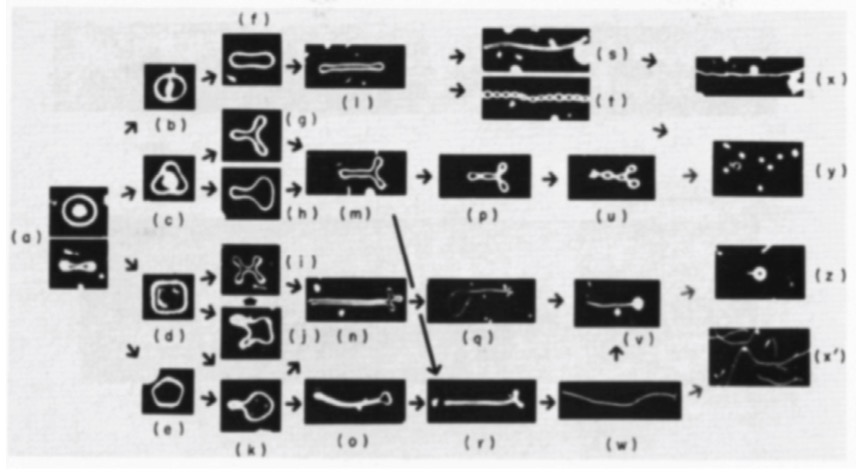
\includegraphics[width=4in]{\MemBio /Pics/GUVPresChange}
\caption{
مسیر‌های مختلفی که یک غشای غول آسای آب نباتی شکل (ستون سمت چپ، زاویه‌ی دوربین از بالا و کنار) که بر اثر تغییر غلظت نمک محیط طی می‌کند تا به شکل خیلی کشیده (ستون سمت راست) در بیاید، را نشان می‌دهد.
}
\label{fig:GUVPresChange}
\end{center}
\end{figure}

GUV همچنین نسبت به تغییرات فشار اسمزی محیط نیز واکنش نشان می‌دهد. مثلا در شکل 
\ref{fig:GUVPresChange}
می‌بینیم که با تغییر غلظت نمک در محیط یک غشایِ لیپیدیِ دارای کلسترول، از شکل اولیه آب نباتیِ 
\LTRfootnote{biconcave}  
شبیه‌ به گلبول قرمز به حالت کشیده و لوله‌ای در می‌آید. در شکل 
\ref{fig:GUVPresChange}
ساختار‌های هندسی میاینی (و در مواردی ناپایدار) مختلفی که غشا طی می‌کند تا از هندسه‌های سمت چپ به هندسه‌های سمت راست برسد، را می‌توان مشاهده کرد.
  
 
 
 
 
 
 
 
 
 
 